Течение Куэтта образуется при относительном движении пластин друг относительно друга с продольной скоростью \(U\),
при этом температуры пластин равны \(T\) и остаются неизменными.
В стационарном состоянии уставливается константный профиль сдвигового напряжения \(p_{xy}\).

Задача переноса тепла ставится для фиксированного отношения температур покоящихся стенок \(T_1>T_2\),
при котором уставливается константный профиль теплового потока \(q_x\).

В качестве дискретного пространства скоростей использовался шар радиусом \(4.3\nu_0\)\footnote
{
	4.3 тепловых скорости достаточно, чтобы обеспечить точность 0.01\% совпадения
	первых тринадцати моментов функции распределения (малой величины) с соответствующими разностными аналогами.
},
равномерно заполненный узлами так, что на радиусе помещалось 16 точек.
Одномерное координатное пространство состояло как минимум из 30 одинаковых кубических ячеек,
при условии что их размер не превышал единицы.

Для взятия интеграла столкновений применялись сетки Коробова размером от 0.1 до 1 млн. точек.
Стационарные значения макропараметров усредненялись на последних 500 временных итераций,
что обеспечивало точность не ниже 0.1\%.

Для ускорения расчётов в качестве начальной функции распределения выбиралось тринадцатимоментное приближение Грэда
\[ 
	\hat{f}_{G13} = \frac{\hat\rho}{(\pi\hat T)^{3/2}}\exp\left(-\frac{c_i^2}{\hat T}\right)
	\left( 1+\frac{\hat p_{ij}c_ic_j}{\hat p\hat T} + \frac4{5}\frac{\hat q_ic_i}{\hat p\hat T}\left(\frac{c_i^2}{\hat T}-\frac5{2}\right) \right),
	\quad c_i = \zeta_i - \hat v_i
\]
с соответствующими точному решению профилями макропараметров.

В задаче Куэтта относительная скорость пластин равнялась \(\hat{U}=0.01\),
и такое же значение отношения температур \(\hat{T}_1/\hat{T}_2\) использовалось в задаче теплопереноса.
Этого достаточно, чтобы обеспечить линейность задачи с точностью порядка 0.01\%.

\subsubsection{Результаты моделирования}

Для задачи Куэтта сравнивались зависимости сдвигового напряжения (рис.~\ref{fig:couette:shear}),
потоков массы (рис.~\ref{fig:couette:flow}) и тепла (рис.~\ref{fig:couette:qflow})
через половину сечения от числа Кнудсена.

Для бесстолкновительного газа
\[ \frac{\hat{p}_{xy}}{\hat{U}} = -\frac1{\sqrt{\pi}} \]
При небольших \(\Kn\) справедливо асимптотическое решение
\[ \frac{\hat{p}_{xy}}{\hat{U}} = \frac{2\hat{\mu}\Kn}{1-\sqrt{\pi}k_0\Kn}. \]
Коэффициенты вязкости \(\hat{\mu}\) и скольжения \(k_0\) для модели твёрдых сфер равны~\cite{Sone2007}
\[ \hat{\mu} = 0.562773, \; k_0 = -1.2540. \]
Отбросив знаменатель, получим гидродинамическое решение \(\hat{p}_{xy} = 2\hat{\mu}\Kn\hat{U}\).
Численные значения точного решения табулированы в~\cite{Sone1990}.

Кроме того, для сравнения представлены некоторые результаты решения модельного уравнения БКВ.
Несмотря на хорошое совпадение модельного решения с точным для значения сдвигового напряжения,
метод БКВ даёт значительную погрешность для потоков массы и тепла~\cite{Sone1990},
поэтому далее не приводятся соответствующие значения.

\begin{figure}
	\centering
	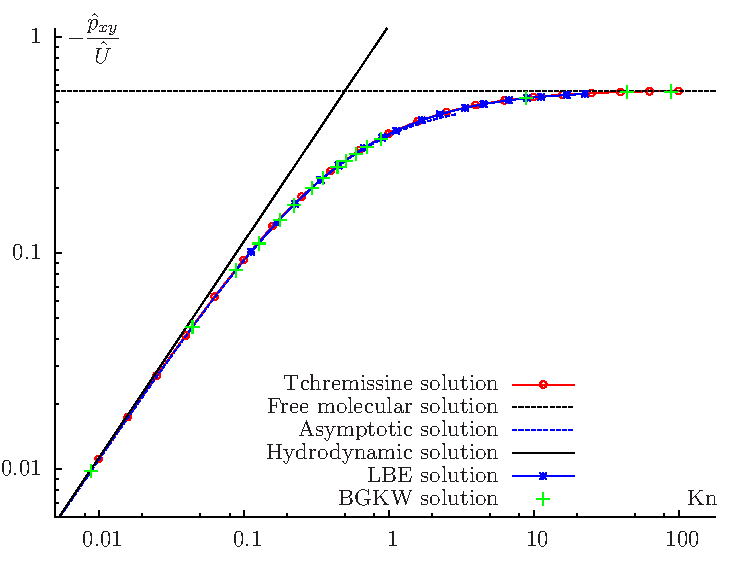
\includegraphics{problems/couette_stress.pdf}
	\caption{Зависимость сдвигового напряжения от числа Кнудсена}\label{fig:couette:shear}
\end{figure}

\begin{figure}
	\centering
	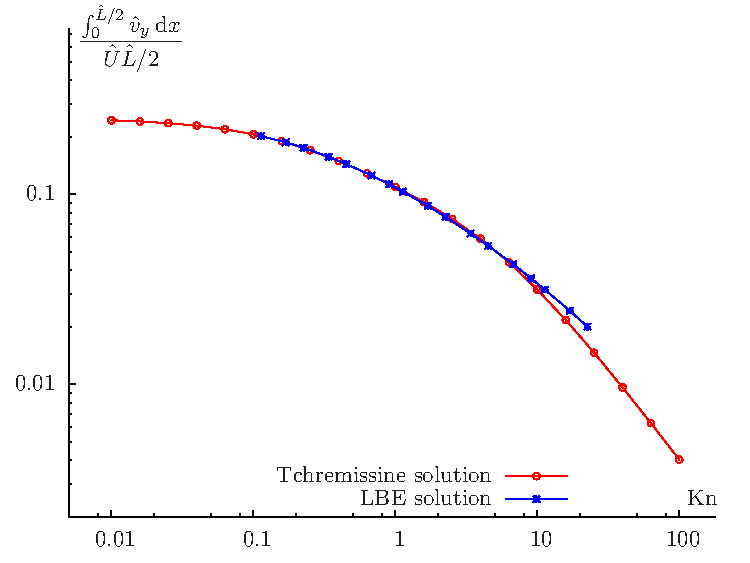
\includegraphics{problems/couette_flow.pdf}
	\caption{Зависимость потока массы через половину сечения от числа Кнудсена}\label{fig:couette:flow}
\end{figure}

\begin{figure}
	\centering
	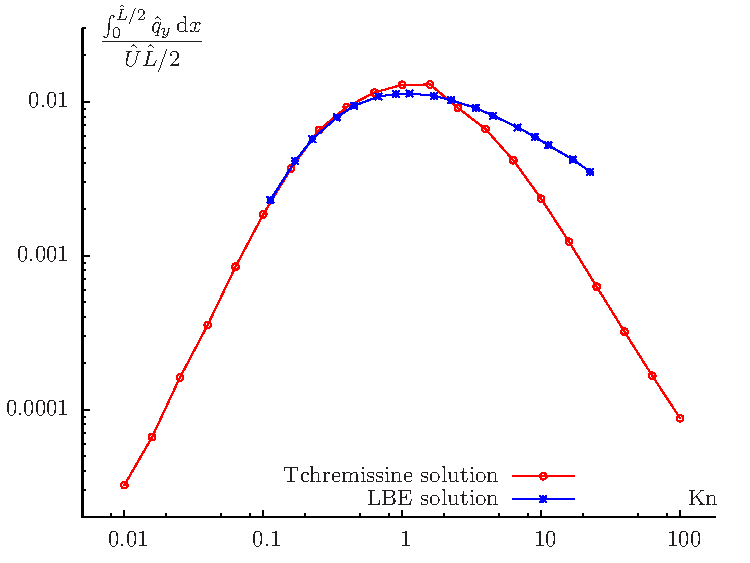
\includegraphics{problems/couette_qflow.pdf}
	\caption{Зависимость потока тепла через половину сечения от числа Кнудсена}\label{fig:couette:qflow}
\end{figure}

На рис.~\ref{fig:couette:shear} наблюдается хорошое совпадение результатов.
Однако для бесстолкновительного газа заметно превышение \(\hat{p}_{xy}\) на 0.61\%,
что может быть обусловлено только ошибкой дискретной аппроксимации функции распределения по скоростному пространству.
При интерполяции полученной кривой на интервале \(\Kn\in[0,0.2]\) асимптотическим решением 
можно произвести подбор параметров нелинейным методом наименьших квадратов.
С его помощью в области континуального описания газа определяется оклонение 
от коэффициентов вязкости (\(+0.83\%\)) и скольжения (\(-1.2\%\)).
Если все полученные значения нормировать на точное значение для бесстолкновительного газа (разделить на 1.0061),
то погрешность в коэффициенте вязкости снижается до \(+0.22\%\), что является уже приемлимым результатом.

На рис.~\ref{fig:couette:flow},~\ref{fig:couette:qflow} для сильно разреженного газа наблюдаются
значительные отклонения, природа которых пока не определена.

Для задачи переноса тепла проанализируем зависимость теплового потока от числа Кнудсена~\ref{fig:heat}.

Для бесстолкновительного газа
\[ \frac{\hat{q}_x}{\hat{T}_1-\hat{T}_2} = -\frac1{\sqrt{\pi}} \]
При небольших \(\Kn\) справедливо асимптотическое решение
\[ \frac{\hat{q}_x}{\hat{T}_1-\hat{T}_2} = -\frac{\hat{\lambda}\Kn}{1+\sqrt{\pi}d_1\Kn}. \]
Коэффициенты теплопроводности \(\hat{\lambda}\) и скачка температуры на стенке \(d_1\) для модели твёрдых сфер равны~\cite{Sone2007}
\[ \hat{\lambda} = 2.129475, \; d_1 = 2.4001. \]
Отбросив знаменатель, получим гидродинамическое решение \(\hat{q}_x = -\hat{\lambda}\Kn(\hat{T}_1-\hat{T}_2)\).
Численные значения точного решения табулированы в~\cite{Sone2007}.

\begin{figure}
	\centering
	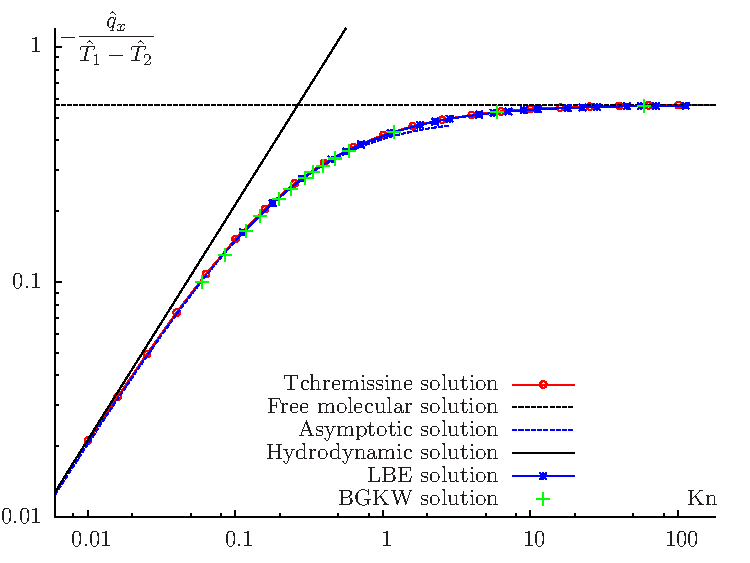
\includegraphics{problems/heat_qflow.pdf}
	\caption{Зависимость теплового потока от числа Кнудсена}\label{fig:heat}
\end{figure}

Как и в задаче о течении Куэтта, на рис.~\ref{fig:heat} видна хорошая сходимость к точному решению,
однако одновременно наблюдаются те же проблемы: завышение значений теплопотока на \(0.63\)\%
для бесстолкновительного газа и значительная ошибка в коэффициенте теплопроводности (\(+2.2\%\)).
По всей видимости, последняя объясняется неточной аппроксимацией угла разлёта сталкивающихся молекул,
в частности, существованием минимально разрешимого угла.

\subsubsection{Исследование погрешности}

Логичным представляется исследование зависимости указанных погрешностей от числа интерполирующих узлов
скоростного пространства. Будем анализировать ошибки аппроксимации задачи переноса тепла.
Для этого коэффициент теплопроводности вычислялся локально в точке \(x_0=\hat L/2\) по формуле
\[ \hat{q_x}(x_0) = -\hat{\lambda}\frac{\D\hat T}{\D x}\bigg|_{x=x_0}. \]

Соответствующие графики в логарифмическом масштабе представлены на рис.~\ref{fig:error}.
Наклон прямых говорит о квадратичной зависимости:
\[ \varepsilon \propto N_\Omega^{-2} \propto V_\Omega^{-2/3}, \]
где \(N_\Omega\) "--- число узлов на радиусе скоростной сетки, \(V_\Omega\) "--- её объём.

При \(N_\Omega = 40\) точность вычисления теплового потока повышается до \(0.1\%\),
а коэффициента теплопроводности только до \(0.5\%\).

\begin{figure}
	\centering
	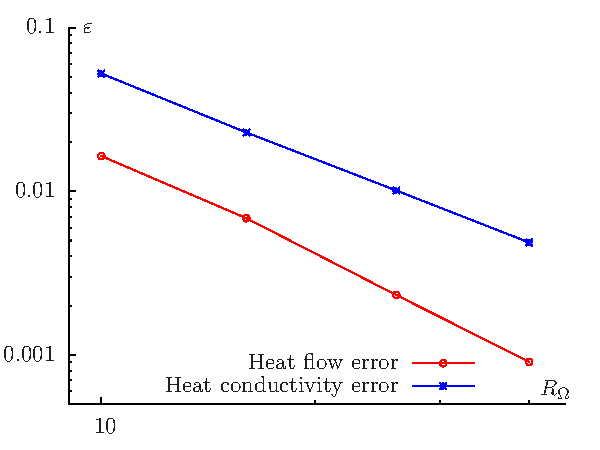
\includegraphics{problems/error.pdf}
	\caption{
		Зависимость от числа узлов на радиусе скоростной сетки погрешностей вычисления 
		теплопотока для бесстолкновительного газа и коэффициента теплопроводности для слаборазреженного газа.
	}\label{fig:error}
\end{figure}

\subsubsection{Резюме}

Показана удовлетворительная сходимость численного решения уравнения Больцмана проекционным методом
простейших одномерных линейных задач: течения Куэтта и переноса тепла, --- к эталонным на основе
линеаризованного уравнения.

Выявлены две проблемы. Во-первых, плохая сходимость погрешности аппроксимации теплового потока по отношению к
объёму используемой памяти. Возможным решением является корректировка всех значений макропараметров
по их отклонению в бесстолкновительном режиме при используемом \(R_\Omega\) от некоторого большего \(R_\Omega\),
при котором результаты можно считать достоверными.

Во-вторых, существенна погрешность в определении коэффициентов вязкости и особенно теплопроводности.
По всей видимости, качественно улучшить аппроксимацию межмолекулярного потенциала позволит лишь использование
более чем двухточечного проекционного метода, который обеспечит точное значение угла разлёта.
